% questions.tex —— 1994 年·全国卷·文科 · 题目内容片段（无答案）
% 由 tools/generate_projects.py 依来源总账自 1994/1994_数学真题_全国文_试题.md 生成，勿手改（改源 MD 后重跑）


\gkpart{数学}

\begin{gktip}
\textbf{来源说明}：依据固定来源 PDF 的原生文字层逐题转录，并对照 400 dpi 渲染与页面内容流逐项核对（上划线、分数线、根号横为矢量短线，不在文字层，须解内容流）。源为 \textbf{XeTeX 重排件（非扫描）}。单页 A3 横向三栏，页脚仅印印刷页码 \textbf{50}；\textbf{源页无大题标题}，题号 1–25 连续；\textbf{无答案页}。

\textbf{标点与字样约定}：① 题号源内为半角句点，本库统一作全角「．」；② 源内句末实心点归一为「。」，其余中文标点归一全角；③ 选项标号源为半角「(A)」，排印统一作全角「（A）」；④ 分数按源竖排真分式，排印用 \(\dfrac{a}{b}\)；⑤ 虚数单位 \(i\) 按源排数学斜体。

\textbf{存疑与登记}（源内异常照录，不推测补正）：① 第 1 题源为 \(\overline{A}\cup\overline{B}\)（补集横线为矢量短线，文字层不含）；② 第 12 题为四幅图象选项（原页四面板，选项字母见图）；③ 第 21 题求最小值、无填空横线，故题组结构为 16–20 填空、21–25 解答。

\textbf{图示}：第 12 题为四幅图象选项（2×2 面板，含 x/y/O/±1 与 (A)–(D) 标注）、第 23 题为棱柱（七顶点标注）；两图均按源 PDF 内容流逐路径重绘（线宽/虚线按源值，标签取源文本中心），不按比例。
\end{gktip}

\begin{question}
\gkti{1}设全集 $I=\{0,1,2,3,4\}$，集合 $A=\{0,1,2,3\}$，集合 $B=\{2,3,4\}$，则 $\overline{A}\cup\overline{B}=$\mbox{（　　）}。

（A）$\{0\}$　　（B）$\{0,1\}$　　（C）$\{0,1,4\}$　　（D）$\{0,1,2,3,4\}$

\end{question}
\begin{question}
\gkti{2}如果方程 $x^2+ky^2=2$ 表示焦点在 $y$ 轴上的椭圆，那么实数 $k$ 的取值范围是\mbox{（　　）}。

（A）$(0,+\infty)$　　（B）$(0,2)$　　（C）$(1,+\infty)$　　（D）$(0,1)$

\end{question}
\begin{question}
\gkti{3}点 $(0,5)$ 到直线 $y=2x$ 的距离是\mbox{（　　）}。

（A）$\dfrac52$　　（B）$\sqrt5$　　（C）$\dfrac32$　　（D）$\dfrac{\sqrt5}{2}$

\end{question}
\begin{question}
\gkti{4}设 $\theta$ 是第二象限的角，则必有\mbox{（　　）}。

（A）$\tan\dfrac\theta2>\cot\dfrac\theta2$　　（B）$\tan\dfrac\theta2<\cot\dfrac\theta2$

（C）$\sin\dfrac\theta2>\cos\dfrac\theta2$　　（D）$\sin\dfrac\theta2<\cos\dfrac\theta2$

\end{question}
\begin{question}
\gkti{5}某种细菌在培养过程中，每20分钟分裂一次（一个分裂为两个）。经过3小时，这种细菌由1个可繁殖成\mbox{（　　）}。

（A）511个　　（B）512个　　（C）1023个　　（D）1024个

\end{question}
\begin{question}
\gkti{6}在下列函数中，以 $\dfrac\pi2$ 为周期的函数是\mbox{（　　）}。

（A）$y=\sin2x+\cos4x$　　（B）$y=\sin2x\cos4x$

（C）$y=\sin2x+\cos2x$　　（D）$y=\sin2x\cos2x$

\end{question}
\begin{question}
\gkti{7}已知正六棱台的上、下底面边长分别为2和4，高为2，则其体积为\mbox{（　　）}。

（A）$32\sqrt3$　　（B）$28\sqrt3$　　（C）$24\sqrt3$　　（D）$20\sqrt3$

\end{question}
\begin{question}
\gkti{8}设 $F_1$ 和 $F_2$ 为双曲线 $\dfrac{x^2}{4}-y^2=1$ 的两个焦点，点 $P$ 在双曲线上且满足 $\angle F_1PF_2=90^\circ$，则 $\triangle F_1PF_2$ 的面积是\mbox{（　　）}。

（A）$1$　　（B）$\dfrac{\sqrt5}{2}$　　（C）$2$　　（D）$\sqrt5$

\end{question}
\begin{question}
\gkti{9}如果复数 $z$ 满足 $|z+i|+|z-i|=2$，那么 $|z+i+1|$ 的最小值是\mbox{（　　）}。

（A）$1$　　（B）$\sqrt2$　　（C）$2$　　（D）$\sqrt5$

\end{question}
\begin{question}
\gkti{10}有甲、乙、丙三项任务，甲需2人承担，乙、丙各需1人承担。从10人中选派4人承担这三项任务，不同的选法共有\mbox{（　　）}。

（A）1260种　　（B）2025种　　（C）2520种　　（D）5040种

\end{question}
\begin{question}
\gkti{11}对于直线 $m,n$ 和平面 $\alpha,\beta$，$\alpha\perp\beta$ 的一个充分条件是\mbox{（　　）}。

（A）$m\perp n,\ m\parallel\alpha,\ n\parallel\beta$

（B）$m\perp n,\ \alpha\cap\beta=m,\ n\subset\alpha$

（C）$m\parallel n,\ n\perp\beta,\ m\subset\alpha$

（D）$m\parallel n,\ m\perp\alpha,\ n\perp\beta$

\Needspace{0.4\textheight}
\end{question}
\begin{question}
\gkti{12}设函数 $f(x)=1-\sqrt{1-x^2}\ (-1\le x\le0)$，则函数 $y=f^{-1}(x)$ 的图象是\mbox{（　　）}。
\nopagebreak[4]
\begin{center}% ../../../1994_全国卷_文科/figures/f1994_national_arts_q12_inverse_graphs.tex — 1994 年·全国卷·文科 第 12 题（四图象选项）
%
% 【来源】`.work/phase4-b19/source/1994全国文.pdf`（SHA-256 68085b2f5b0285e127f63c87f6737434fddb156cbc4689b8957c2a4be4bb1bda），第 1 页；
%   内容流逐路径照录，本地坐标 = 页面坐标 − (458.700,608.330)，1 单位 = 1 TeX pt。
%   每个 m 子路径独立起笔；线宽/虚线按内容流原值；标签取 pdftotext -bbox 中心。
%
% 元素计数：24 路径＋24 标签
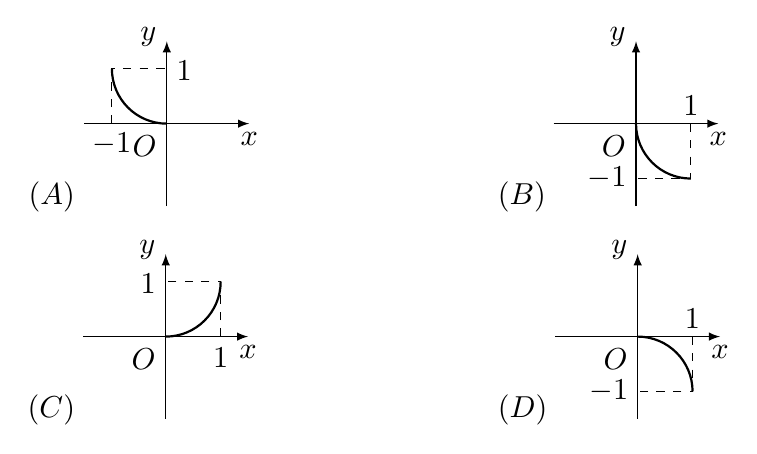
\begin{tikzpicture}[x=1pt, y=1pt,
    every node/.style={inner sep=0pt, font=\fontsize{10.5pt}{12.6pt}\selectfont}]
  \draw[line width=0.398pt] (0.378,106.710) -- (56.319,106.710);
  \fill[line width=1.0pt] (59.906,106.710) .. controls (58.843,106.909) and (57.116,107.507) .. (55.921,108.204) -- (55.921,105.216) .. controls (57.116,105.913) and (58.843,106.511) .. (59.906,106.710);
  \draw[line width=0.398pt] (30.142,76.946) -- (30.142,132.887);
  \fill[line width=1.0pt] (30.142,136.474) .. controls (29.943,135.411) and (29.345,133.684) .. (28.648,132.489) -- (31.636,132.489) .. controls (30.939,133.684) and (30.341,135.411) .. (30.142,136.474);
  \draw[line width=0.398pt, dash pattern=on 2.989pt off 2.989pt] (10.299,106.710) -- (10.299,126.553) -- (30.142,126.553);
  \draw[line width=0.797pt] (30.142,106.710) .. controls (19.183,106.710) and (10.299,115.594) .. (10.299,126.553);
  \draw[line width=0.398pt] (169.928,106.710) -- (225.869,106.710);
  \fill[line width=1.0pt] (229.456,106.710) .. controls (228.393,106.909) and (226.666,107.507) .. (225.471,108.204) -- (225.471,105.216) .. controls (226.666,105.913) and (228.393,106.511) .. (229.456,106.710);
  \draw[line width=0.398pt] (199.692,76.946) -- (199.692,132.887);
  \fill[line width=1.0pt] (199.692,136.474) .. controls (199.493,135.411) and (198.895,133.684) .. (198.198,132.489) -- (201.186,132.489) .. controls (200.489,133.684) and (199.891,135.411) .. (199.692,136.474);
  \draw[line width=0.398pt, dash pattern=on 2.989pt off 2.989pt] (219.535,106.710) -- (219.535,86.867) -- (199.692,86.867);
  \draw[line width=0.797pt] (199.692,106.710) .. controls (199.692,95.751) and (208.576,86.867) .. (219.535,86.867);
  \draw[line width=0.398pt] (-0.004,29.761) -- (55.937,29.761);
  \fill[line width=1.0pt] (59.524,29.761) .. controls (58.461,29.960) and (56.734,30.558) .. (55.539,31.255) -- (55.539,28.267) .. controls (56.734,28.964) and (58.461,29.562) .. (59.524,29.761);
  \draw[line width=0.398pt] (29.760,-0.003) -- (29.760,55.938);
  \fill[line width=1.0pt] (29.760,59.525) .. controls (29.561,58.462) and (28.963,56.735) .. (28.266,55.540) -- (31.254,55.540) .. controls (30.557,56.735) and (29.959,58.462) .. (29.760,59.525);
  \draw[line width=0.398pt, dash pattern=on 2.989pt off 2.989pt] (49.603,29.761) -- (49.603,49.604) -- (29.760,49.604);
  \draw[line width=0.797pt] (29.760,29.761) .. controls (40.719,29.761) and (49.603,38.645) .. (49.603,49.604);
  \draw[line width=0.398pt] (170.516,29.761) -- (226.457,29.761);
  \fill[line width=1.0pt] (230.044,29.761) .. controls (228.981,29.960) and (227.254,30.558) .. (226.059,31.255) -- (226.059,28.267) .. controls (227.254,28.964) and (228.981,29.562) .. (230.044,29.761);
  \draw[line width=0.398pt] (200.280,-0.003) -- (200.280,55.938);
  \fill[line width=1.0pt] (200.280,59.525) .. controls (200.081,58.462) and (199.483,56.735) .. (198.786,55.540) -- (201.774,55.540) .. controls (201.077,56.735) and (200.479,58.462) .. (200.280,59.525);
  \draw[line width=0.398pt, dash pattern=on 2.989pt off 2.989pt] (220.123,29.761) -- (220.123,9.918) -- (200.280,9.918);
  \draw[line width=0.797pt] (200.280,29.761) .. controls (211.239,29.761) and (220.123,20.877) .. (220.123,9.918);
  \node[anchor=center] at (23.490,137.970) {$y$};
  \node[anchor=center] at (59.910,101.230) {$x$};
  \node[anchor=center] at (22.150,98.570) {$O$};
  \node[anchor=center] at (36.470,125.900) {$1$};
  \node[anchor=center] at (10.300,99.500) {$-1$};
  \node[anchor=center] at (-11.430,80.070) {$(A)$};
  \node[anchor=center] at (193.040,137.970) {$y$};
  \node[anchor=center] at (229.460,101.230) {$x$};
  \node[anchor=center] at (191.700,98.570) {$O$};
  \node[anchor=center] at (219.540,113.140) {$1$};
  \node[anchor=center] at (189.280,87.180) {$-1$};
  \node[anchor=center] at (158.430,80.070) {$(B)$};
  \node[anchor=center] at (23.110,61.020) {$y$};
  \node[anchor=center] at (59.520,24.280) {$x$};
  \node[anchor=center] at (21.760,21.620) {$O$};
  \node[anchor=center] at (23.440,48.950) {$1$};
  \node[anchor=center] at (49.600,22.030) {$1$};
  \node[anchor=center] at (-11.570,3.120) {$(C)$};
  \node[anchor=center] at (193.630,61.020) {$y$};
  \node[anchor=center] at (230.040,24.280) {$x$};
  \node[anchor=center] at (192.280,21.620) {$O$};
  \node[anchor=center] at (220.120,36.190) {$1$};
  \node[anchor=center] at (189.870,10.230) {$-1$};
  \node[anchor=center] at (158.730,3.120) {$(D)$};
\end{tikzpicture}
%
% 【自验结果】逐路径照录；探针编译 0 警告。
\end{center}
\nopagebreak[4]
\end{question}
\begin{question}
\gkti{13}已知过球面上 $A,B,C$ 三点的截面和球心的距离等于球半径的一半，且 $AB=BC=CA=2$，则球面面积是\mbox{（　　）}。

（A）$\dfrac{16\pi}{9}$　　（B）$\dfrac{8\pi}{3}$　　（C）$4\pi$　　（D）$\dfrac{64\pi}{9}$

\end{question}
\begin{question}
\gkti{14}如果函数 $y=\sin2x+a\cos2x$ 的图象关于直线 $x=-\dfrac\pi8$ 对称，那么 $a=$\mbox{（　　）}。

（A）$\sqrt2$　　（B）$-\sqrt2$　　（C）$1$　　（D）$-1$

\end{question}
\begin{question}
\gkti{15}定义在 $(-\infty,+\infty)$ 上的任意函数 $f(x)$ 都可以表示成一个奇函数 $g(x)$ 和一个偶函数 $h(x)$ 之和。如果 $f(x)=\lg(10^x+1)$，$x\in(-\infty,+\infty)$，那么\mbox{（　　）}。

（A）$g(x)=x,\quad h(x)=\lg(10^x+10^{-x}+2)$

（B）$g(x)=\dfrac12[\lg(10^x+1)+x],\quad h(x)=\dfrac12[\lg(10^x+1)-x]$

（C）$g(x)=\dfrac{x}{2},\quad h(x)=\lg(10^x+1)-\dfrac{x}{2}$

（D）$g(x)=-\dfrac{x}{2},\quad h(x)=\lg(10^x+1)+\dfrac{x}{2}$

\end{question}
\begin{question}
\gkti{16}在 $(3-x)^7$ 的展开式中，$x^5$ 的系数是\underline{\qquad\qquad}。（用数字作答）

\end{question}
\begin{question}
\gkti{17}抛物线 $y^2=8-4x$ 的准线方程是\underline{\qquad\qquad}，圆心在该抛物线的顶点且与其准线相切的圆的方程是\underline{\qquad\qquad}。

\end{question}
\begin{question}
\gkti{18}已知 $\sin\theta+\cos\theta=\dfrac15$，$\theta\in(0,\pi)$，则 $\cot\theta$ 的值是\underline{\qquad\qquad}。

\end{question}
\begin{question}
\gkti{19}设圆锥底面圆周上两点 $A,B$ 间的距离为2，圆锥顶点到直线 $AB$ 的距离为 $\sqrt3$，$AB$ 和圆锥的轴的距离为1，则该圆锥的体积为\underline{\qquad\qquad}。

\end{question}
\begin{question}
\gkti{20}在测量某物理量的过程中，因仪器和观察的误差，使得 $n$ 次测量分别得到 $a_1,a_2,\ldots,a_n$，共 $n$ 个数据。我们规定所测量物理量的“最佳近似值”$a$ 是这样一个量：与其他近似值比较，$a$ 与各数据的差的平方和最小。依此规定，从 $a_1,a_2,\ldots,a_n$ 推出的 $a=$\underline{\qquad\qquad}。

\end{question}
\begin{question}
\gkti{21}求函数
\nopagebreak[4]
\[
y=\frac{\sin3x\sin^3x+\cos3x\cos^3x}{\cos^2 2x}+\sin2x
\]
的最小值。

\end{question}
\begin{question}
\gkti{22}已知函数 $f(x)=\log_a x\ (a>0\text{\text{且}}a\ne1,\ x\in\mathbb R_+)$。若 $x_1,x_2\in\mathbb R_+$，判断 $\dfrac12[f(x_1)+f(x_2)]$ 与 $f\!\left(\dfrac{x_1+x_2}{2}\right)$ 的大小，并加以证明。

\Needspace{0.4\textheight}
\end{question}
\begin{question}
\gkti{23}如图，已知 $A_1B_1C_1-ABC$ 是正三棱柱，$D$ 是 $AC$ 中点。

（1） 证明：$AB_1\parallel\text{\text{平面} }DBC_1$；

（2） 假设 $AB_1\perp BC_1$，$BC=2$，求线段 $AB_1$ 在侧面 $B_1BCC_1$ 上的射影长。
\nopagebreak[4]
\begin{center}% ../../../1994_全国卷_文科/figures/f1994_national_arts_q23_prism.tex — 1994 年·全国卷·文科 第 23 题（棱柱）
%
% 【来源】`.work/phase4-b19/source/1994全国文.pdf`（SHA-256 68085b2f5b0285e127f63c87f6737434fddb156cbc4689b8957c2a4be4bb1bda），第 1 页；
%   内容流逐路径照录，本地坐标 = 页面坐标 − (1034.000,477.000)，1 单位 = 1 TeX pt。
%   每个 m 子路径独立起笔；线宽/虚线按内容流原值；标签取 pdftotext -bbox 中心。
%
% 元素计数：实线 8 段＋虚线 5 段＋7 标签
% 主会话 2026-10-23 审校修正：C₁ 原在 (19.9,48.8)，下标被实线 AB₁ 与虚线 C₁B₁ 切穿，收进左面三角形内并离顶点 11pt（15.0,54.0）；其余照源。
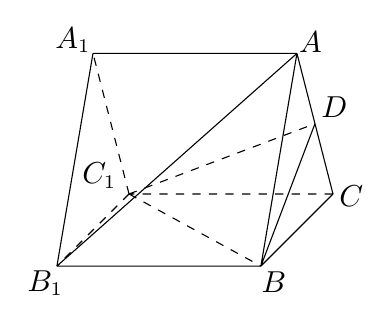
\begin{tikzpicture}[x=1pt, y=1pt,
    every node/.style={inner sep=0pt, font=\fontsize{10.5pt}{12.6pt}\selectfont}]
  \draw[line width=0.398pt] (86.405,98.269) -- (73.378,21.413) (99.432,47.467) -- (73.378,21.413) (12.701,98.269) -- (-0.326,21.413) (73.378,21.413) -- (-0.326,21.413) (86.405,98.269) -- (12.701,98.269) (92.919,72.868) -- (73.378,21.413) (86.405,98.269) -- (-0.326,21.413) (86.405,98.269) -- (99.432,47.467);
  \draw[line width=0.398pt, dash pattern=on 2.989pt off 2.989pt] (25.728,47.467) -- (12.701,98.269) (25.728,47.467) -- (-0.326,21.413) (25.728,47.467) -- (73.377,21.413) (25.728,47.467) -- (92.918,72.868) (99.432,47.467) -- (25.728,47.467);
  \node[anchor=center] at (5.500,103.000) {$A_1$};
  \node[anchor=center] at (91.340,102.350) {$A$};
  \node[anchor=center] at (-4.500,15.200) {$B_1$};
  \node[anchor=center] at (78.050,15.630) {$B$};
  \node[anchor=center] at (15.000,54.000) {$C_1$};
  \node[anchor=center] at (106.030,46.620) {$C$};
  \node[anchor=center] at (99.900,78.900) {$D$};
\end{tikzpicture}
%
% 【自验结果】逐路径照录；探针编译 0 警告。
\end{center}
\nopagebreak[4]
\end{question}
\begin{question}
\gkti{24}已知直角坐标平面上点 $Q(2,0)$ 和圆 $C:x^2+y^2=1$，动点 $M$ 到圆 $C$ 的切线长与 $|MQ|$ 的比等于常数 $\lambda\ (\lambda>0)$。求动点 $M$ 的轨迹方程，说明它表示什么曲线。

\end{question}
\begin{question}
\gkti{25}设数列 $\{a_n\}$ 的前 $n$ 项和为 $S_n$，若对于所有的自然数 $n$，都有
\nopagebreak[4]
\[
S_n=\frac{n(a_1+a_n)}{2},
\]
证明 $\{a_n\}$ 是等差数列。

\end{question}